\subjectPresentation{1}{Introduction}{color1}

\subjectDevelopment{Context}{
    \centering
    \begin{tikzpicture}[node distance=3cm]
        \node[circle, draw, fill=color2!20, minimum size=3cm, align=center, text width=2cm] (a) {Analysis of the \\ USA Census};
        \node[circle, draw, fill=color3!20, minimum size=3cm, align=center, text width=2cm] (b) [right=of a] {Weather\\Forecasting};
    \end{tikzpicture}
    \vfill
    What's the importance of these themes? Why do we use Machine Learning to do these tasks? And how they are linked?
}{color1}

\subjectDevelopment{First subject: The USA Census}{
\begin{columns}[T]
    \begin{column}{0.5\textwidth}

        \begin{itemize}
            \item Data of Analysis: Folktables dataset
            \item Application: Prediction of a person's income (higher and lower income)
            \item \textbf{Objective: Undestand patterns on the population, that can be used by banks (e.g. loan release)}
        \end{itemize}
        
    \end{column}
    \begin{column}{0.5\textwidth}
        \centering
        \scriptsize
        \begin{table}[h]
            \caption{Folktables Features}
            \begin{tabular}{p{1.2cm}p{1.8cm}}
                \hline
                \textbf{Feature} & \textbf{Description} \\
                \hline
                AGEP & Age \\
                COW & Worker Class \\
                SCHL & Education \\
                MAR & Marital Status \\
                OCCP & Occupation \\
                POBP & Birth Place \\
                RELP & Relationship \\
                WKHP & Work Hours \\
                SEX & Sex \\
                RAC1P & Race \\
                \hline
            \end{tabular}
        \end{table}
    \end{column}
\end{columns}
}{color1}

\subjectDevelopment{Second subject: Weather forecasting}{
\begin{columns}[T]
    \begin{column}{0.5\textwidth}
        \begin{itemize}
            \item Data of Analysis: Titan dataset (AROME and ARPÈGE images)
            \item Application: Prediction of the weather (variables of temperature, wind, geopotencial, humidity, ...) in the next hour
            \item \textbf{Objective: 100x Faster weather predictions, less computational resources, investigation of extreme climate events}
        \end{itemize}
    \end{column}

    \begin{column}{0.5\textwidth}
        \centering
        \scriptsize
        
        \begin{figure}[h]
            % Imagens muito pequenas
            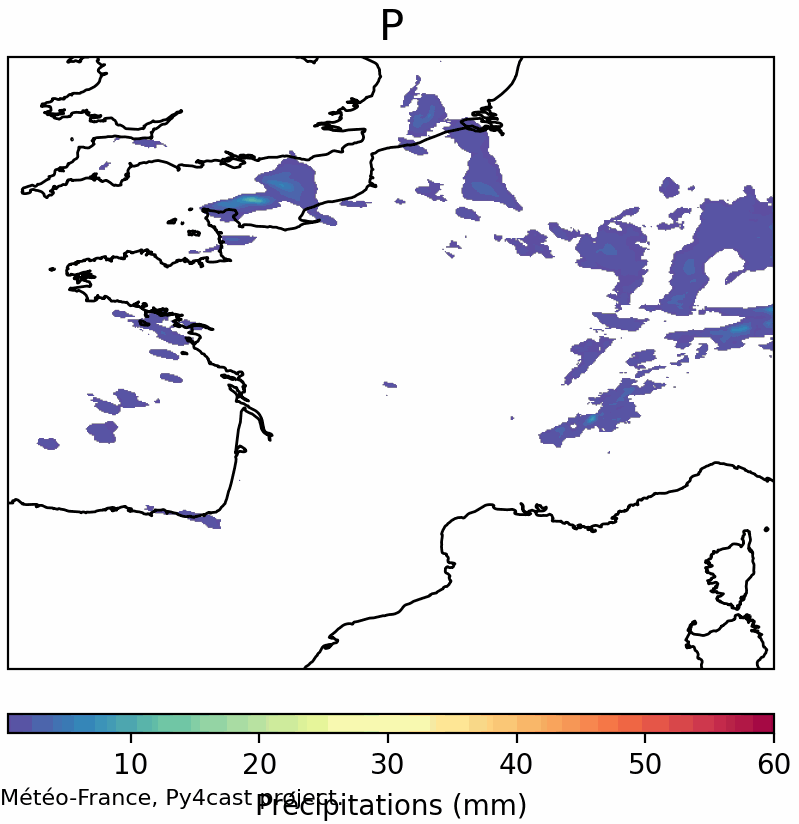
\includegraphics[width=0.4\textwidth]{Images/titan_data_examples/2023111700_feature_aro_tp_0m.png}
            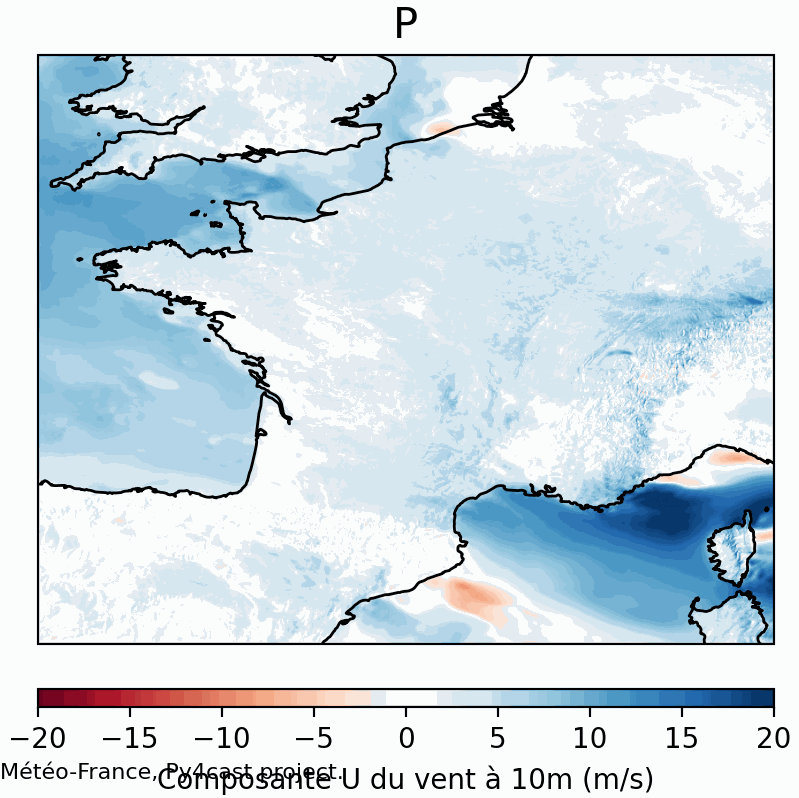
\includegraphics[width=0.4\textwidth]{Images/titan_data_examples/2023111700_feature_aro_u10_10m.png}
            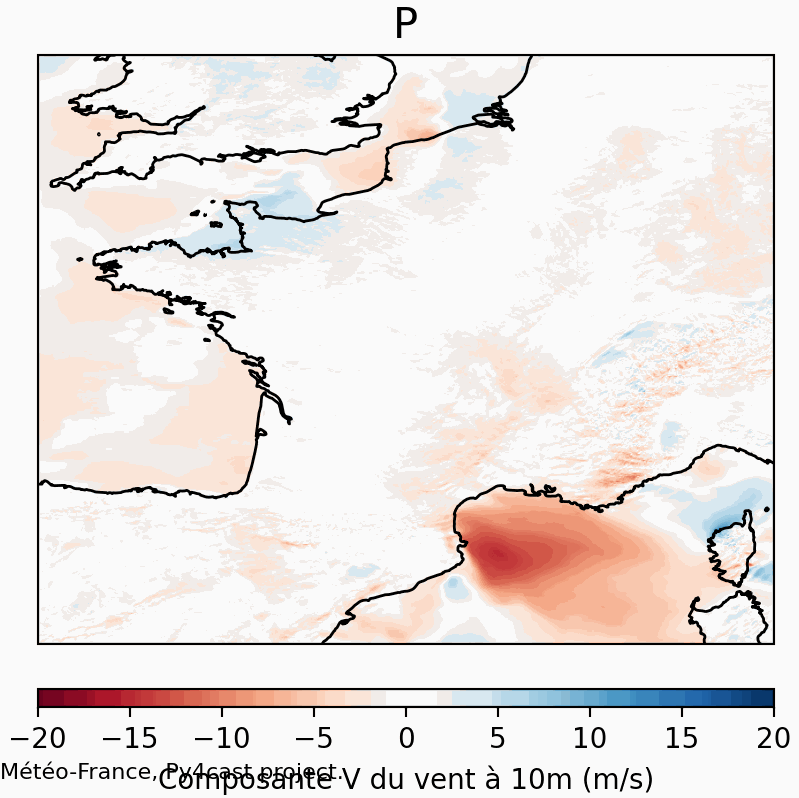
\includegraphics[width=0.4\textwidth]{Images/titan_data_examples/2023111700_feature_aro_v10_10m.png}
            
            \vspace{0.1cm}
            \begin{minipage}{0.4\textwidth}
                \centering\tiny TP 0m
            \end{minipage}
            \hfill
            \begin{minipage}{0.4\textwidth}
                \centering\tiny U10 10m
            \end{minipage}
            \hfill
            \begin{minipage}{0.4\textwidth}
                \centering\tiny V10 10m
            \end{minipage}
            
            \vspace{0.1cm}
            \caption{\scriptsize Titan image channels}
        \end{figure}
    \end{column}
\end{columns}
}{color1}

\subjectDevelopment{What's eXplainable AI (XAI)}{
    The XAI is a domain that gives tools to increase the user's \textbf{interpretability and trust} on the results of Artificial Intelligence (AI) models.

    \vfill

    Critical domains require investigation...

    \vfill

    \begin{tikzpicture}[node distance=3cm]
        \node[circle, draw, fill=color2!20, minimum size=3cm, align=center, text width=2cm] (a) {Identify bias \\ on \\ USA Census};
        \node[circle, draw, fill=color3!20, minimum size=3cm, align=center, text width=2cm] (b) [right=of a] {Increase trust \\ on weather \\ forecasting};
    \end{tikzpicture}
}{color1}

\subjectDevelopment{Main ideas explored}{
  \begin{enumerate}
    \item Understanding the results of the AI “black boxes”
    \begin{enumerate}
      \item The need to develop adapted eXplainable AI (XAI) techniques
      \item Verify that the model's results are made with the "right reasons"
    \end{enumerate}
    \item Adaptable XAI techniques (low and high dimensional data)
    \begin{enumerate}
      \item Used for classification and regression tasks
      \item Explanations that are representable
    \end{enumerate}
  \end{enumerate}
}{color1}

\subjectDevelopment{XAI techniques}{
    \begin{itemize}
        \item SHAP, Lime (perturbation-based)
        \item \textbf{Anchors} (example-based)
        \item Smooth Gradient, Integrated Gradient (gradient-based)
    \end{itemize}
}{color1}

\subjectDevelopment{Why exploring Anchors?}{
    \centering
    Explanations with a promise of being compact and representable, other than being a high precision result, and human understandable!

    \vfill

    \textit{More precise for low-dimensional data, and adaptable for high-dimensional data.}
}{color1}

\subjectDevelopment{Diving deeper on Anchors}{
    Considering a binary classifier $f : \mathcal{X} \rightarrow \{0, 1\}$. For a given instance $x$, the objective is to find a predicate \textbf{$A$ that explains the prediction $f(x)$ by identifying a minimal set of decisive features}.

    A predicate $A$ is deemed a valid anchor if it meets a precision threshold, meaning it \textbf{guarantees the model's output is consistent under local perturbation}. Precision is formally defined as:
    \begin{equation}
    \text{prec}(A) = \mathbb{E}_{D(z|A)} [\mathbf{1}_{f(x) = f(z)}]
    \label{eq:prec-anchors}
    \end{equation}
    where $D(\cdot|A)$ is the conditional distribution of inputs satisfying $A$. The anchor condition is satisfied with high confidence if $P(\text{prec}(A) \geq \tau) \geq 1 - \delta$.
}{color1}
\subjectDevelopment{Diving deeper on Anchors}{
    To select the most impactful and parsimonious explanation for end-users, the method introduces a coverage measure. The coverage of \textbf{$A$ is defined as the probability that the predicate holds under the data distribution}:
    \begin{equation}
    \text{cov}(A) = \mathbb{E}_{D(z)} [A(z)]
    \label{eq:cov-anchors}
    \end{equation}

    For a given data distribution $D$, parameters $\tau$ and $\delta$, the optimal anchor is the one with maximum coverage subject to the precision constraint:
    \begin{equation}
    \arg \max_{A} {\text{cov}(A) \mid P(\text{prec}(A) \geq \tau) \geq 1 - \delta }
    \label{eq:max-cov-anchors}
    \end{equation}
}{color1}